% !TEX TS-program = pdflatex
% !TEX encoding = UTF-8 Unicode

% This is a simple template for a LaTeX document using the "article" class.
% See "book", "report", "letter" for other types of document.

\documentclass[11pt]{article} % use larger type; default would be 10pt

\usepackage[utf8]{inputenc} % set input encoding (not needed with XeLaTeX)

%%% Examples of Article customizations
% These packages are optional, depending whether you want the features they provide.
% See the LaTeX Companion or other references for full information.

%%% PAGE DIMENSIONS
\usepackage{geometry} % to change the page dimensions
\geometry{a4paper} % or letterpaper (US) or a5paper or....
% \geometry{margin=2in} % for example, change the margins to 2 inches all round
% \geometry{landscape} % set up the page for landscape
%   read geometry.pdf for detailed page layout information

\usepackage{graphicx} % support the \includegraphics command and options

% \usepackage[parfill]{parskip} % Activate to begin paragraphs with an empty line rather than an indent

%%% PACKAGES
\usepackage{booktabs} % for much better looking tables
\usepackage{array} % for better arrays (eg matrices) in maths
\usepackage{paralist} % very flexible & customisable lists (eg. enumerate/itemize, etc.)
\usepackage{verbatim} % adds environment for commenting out blocks of text & for better verbatim
\usepackage{subfig} % make it possible to include more than one captioned figure/table in a single float
% These packages are all incorporated in the memoir class to one degree or another...

\usepackage{program} % code listings.

%%% HEADERS & FOOTERS
\usepackage{fancyhdr} % This should be set AFTER setting up the page geometry
\pagestyle{fancy} % options: empty , plain , fancy
\renewcommand{\headrulewidth}{0pt} % customise the layout...
\lhead{}\chead{}\rhead{}
\lfoot{}\cfoot{\thepage}\rfoot{}

%%% SECTION TITLE APPEARANCE
\usepackage{sectsty}
\allsectionsfont{\sffamily\mdseries\upshape} % (See the fntguide.pdf for font help)
% (This matches ConTeXt defaults)

%%% ToC (table of contents) APPEARANCE
\usepackage[nottoc,notlof,notlot]{tocbibind} % Put the bibliography in the ToC
\usepackage[titles,subfigure]{tocloft} % Alter the style of the Table of Contents
\renewcommand{\cftsecfont}{\rmfamily\mdseries\upshape}
\renewcommand{\cftsecpagefont}{\rmfamily\mdseries\upshape} % No bold!

%%% END Article customizations

%%% The "real" document content comes below...

\title{CS211 Wordladder Assignment}
\author{Jacob Smith <jas32>}
%\date{} % Activate to display a given date or no date (if empty),
         % otherwise the current date is printed 

\begin{document}
\maketitle

\section{Program Invocation}

\subsection{Generation mode}
The program can be invoked in generation mode with \texttt{java -jar wordladder.jar <start word> <depth>}. This produces a random word ladder with \texttt{start word} as the first entry out to the depth specified by \texttt{depth} assuming such a word ladder is possible with the dictionary included.

\subsection{Discovery mode}
The program can be invoked in discovery mode with \texttt{java -jar wordladder.jar <start word> <end word>}. This produces a word ladder with the given start and end points. It will attempt to construct the shortest word ladder possible using the included dictionary.

\section{Class Schema (figure \ref{fig:ClassDiagram}) }

\begin{figure}[h!!]
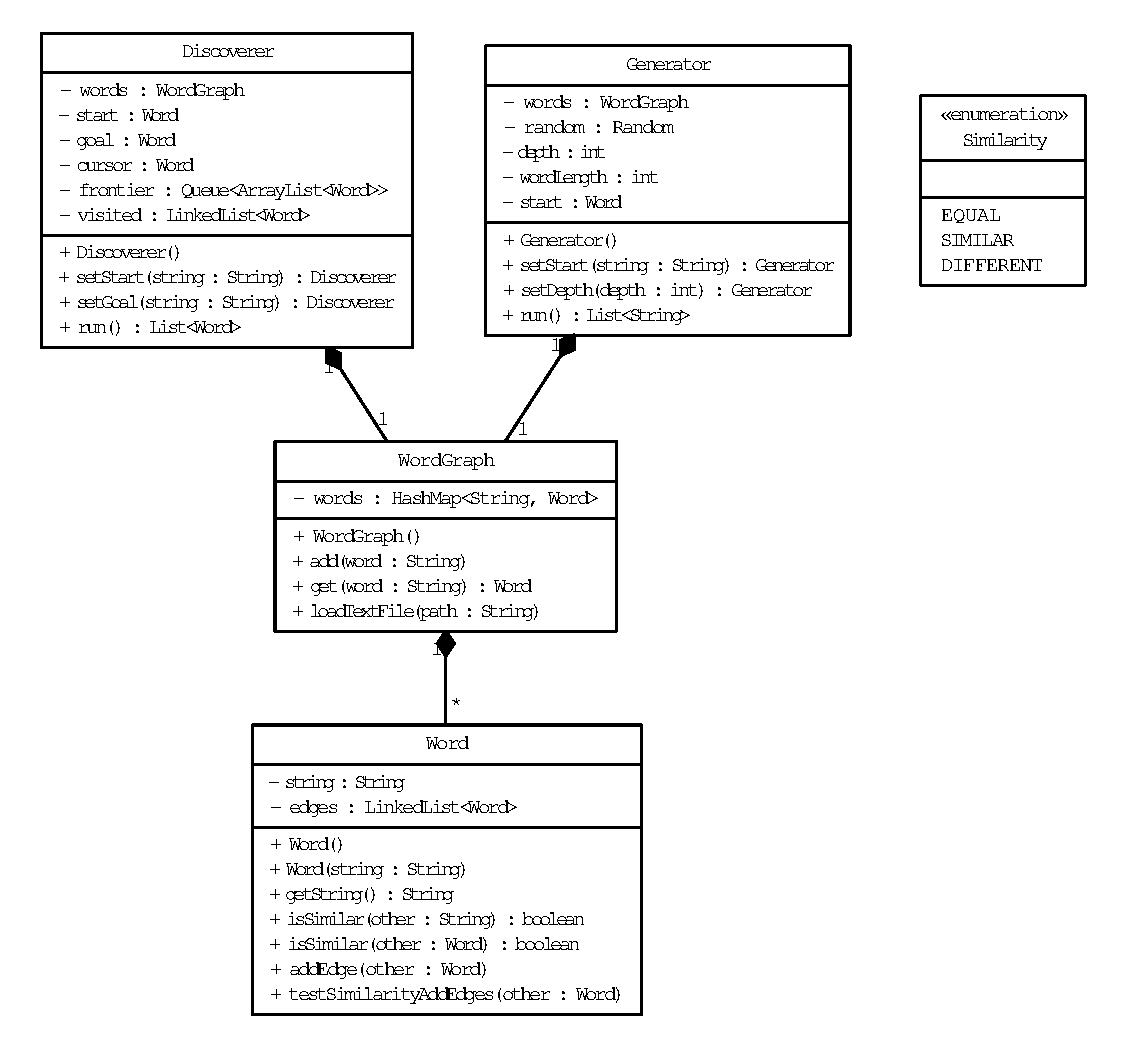
\includegraphics[width=\textwidth]{ClassDiagram}
\caption{Class Diagram for uk.ac.aber.cs211.wordladder package.}
\label{fig:ClassDiagram}
\end{figure}

The \texttt{Word} object encapsulates a word as a part of a graph whose edges represent valid transitions to 'similar' words (ie those with exactly one different character). These edges are stored as a \texttt{LinkedList<Word>} (the many:many aggregation is not pictured). A linked list is used as this structure is typically very small and both Generator and Discoverer need to remove edges that are no longer promising frontiers for expansion. The method \texttt{testSimilarityAddEdges(Word)} compares a word with this one, if they are 'similar' it adds a pair of edges between them (one in each direction). It is this method which is used to populate the graph.

\texttt{WordGraph} stores the dictionary of words known to the program. It may be interrogated for a particular \texttt{Word} using the method \texttt{get(String)}. Words should be added to the dictionary first using \texttt{add(String)}, this behaves as a factory for new \texttt{Word} objects - populating their edges.

\texttt{Generator} and \texttt{Discoverer} are the entry-points into the package. Their setters are used to initialise them (and their \texttt{WordGraph}) before being \texttt{run()}. Their algorithms (and thus attributes) are described in more detail in the next section. Both classes modify their \texttt{WordGraph} during operation - a new one must be built (by calling their setters) before it can be run again.

\section{Algorithms and Search Strategy}

\subsection{Random Wordladder Generation (figure \ref{fig:GeneratorAlgorithm}) } 
$depth$ and $start$ are both parameters, representing the size of the desired word ladder and the first element respectively. $array$ is an empty array or dynamic array with length at least equal to $depth$.

\begin{figure}[h!!]
\caption{Algorithm for random walk taken by Generator.}
\begin{program}
\BEGIN
cursor := start
|append | cursor | to | array
\FOR i := 1 \TO depth \DO
	edges := | get | edges | from | cursor \rcomment{Expand edges}
	\FOR seen | in | array \DO
		|remove | seen | from | edges  \rcomment{Prune visited elements}
	\OD
	\IF edges | is empty| \THEN 
		i := i - 2 \rcomment{Backtrack}
		cursor := |last in | array
		|remove last in |array
	\ELSE
		cursor := |random from | edges \rcomment{Take a random walk}
		|append | cursor | to | array 
	\FI
\OD
\IF array | length equals | depth | |\THEN
	|return | array 
\ELSE
	|return |null \rcomment{No ladder is possible}
\FI
	
\END	
\end{program}

\label{fig:GeneratorAlgorithm}
\end{figure}

\subsection{Algorithm to find word ladder linking two words (figure \ref{fig:DiscoverAlgorithm}).}
$queue$ is a queue of dynamic arrays, initialised with the start word as a singleton array. Arrays are used to represent possible solutions as it is necessary to copy failed solutions (to propose new solutions) and a contiguous block of memory can be copied in fewer low-level operations than a non-contiguous block of memory. $goal$ is simply the destination the word ladder must reach as a parameter. $list$ is an empty list, into which any 'visited' words will be placed, so that they will not be considered in any future solutions.


\begin{figure}[h!!]
\caption{Algorithm to solve a word ladder given a start and end word of equal length, using Breadth First Search.}
\begin{program}
\BEGIN
\WHILE queue| is not empty|\DO
	solution := |pop from |queue \rcomment{Get the next potential solution.}
	cursor := |last in |solution

	\IF cursor| equals |goal | |\THEN
		|return |solution \rcomment{Return the first valid solution found.}
	\FI
	
	edges := |get |edges| from |cursor
	\FOR seen| in |list \DO
		|remove |seen| from |edges \rcomment{Prune visited nodes from search.}
	\OD

	\FOR word| in |edges \DO
		new solution := |copy |solution \rcomment{Propose a new solution.}
		|append |word| to |new solution
		|append |word| to |list \rcomment{Consider no word more than once.}
		|push |new solution| to queue| \rcomment{Push it to the back of the queue.}
	\OD

	|return |null \rcomment{No solution is possible with the current dictionary.}
\OD
\END
\end{program}
\label{fig:DiscoverAlgorithm}
\end{figure}

\end{document}
